\chapter{Additive manufacturing}


\section{Powder Bed Fusion with Laser Beam of Metals (PBF-LB/M)}

Powder Bed Fusion with Laser Beam (PBF-LB) of Metals is an additive manufacturing  technique.
It is used to create complex metal parts by selectively melting and fusing metal powder layer by layer 
using a high-powered laser.

Process:
\begin{enumerate}
    \item A thin layer of metal powder is spread on the bed 
    \item Laser melts the powder in the desired shape
    \item A new layer is deposited
    \item Steps 1 \pd 3 repeats until the shape is complete
    \item Cooling and solidification
    \item Post-Processing
\end{enumerate}

Advantages of laser 3D printing are:
\begin{itemize}
    \item Complex geometries
    \item High efficiency with material
    \item Strong parts
    \item Customization \pd low quantity or unique products
\end{itemize}

Same process can be done with polymer materials \pd Powder Bed Fusion with Laser Beam of \textbf{Polymers} (PBF-LB/P).

The interaction between the material and laser is a combination of \textit{heat } and \textit{deep conduction welding} - depends on the speed and 
power of the laser processing. 

Physical interactions between the laser and material are absorption, heat conduction, phase transition \dots

Particle powder properties - shape, size, distribution, chemical composition and moisture - also influence the process and 
end product. 

Applications for PBF are creating unique products (implants) and product that can not be 
created with other techniques (e.g: internal cooling chanels).

When working with polymers, we have to \textbf{preheat the  polymer material} to temperatures above 
the crystallization temperature. We can only use a small range of polymers. 


\section{Stereolithography}

Stereolithography is a process in which we use a liquid polymer (or monomer) and 
harden it layer by layer with a laser. The platform lowers each layer. 
We mostly use duroplasts.

\section{2P-polymerization}
We can create smaller shapes using nonlinear absorption. 

\section{Directed energy deposition}
Laser beam is used to melt the deposited material on the base. Figure \ref{fig:ded} show the nozzle.

\begin{figure}[h!]
    \centering
    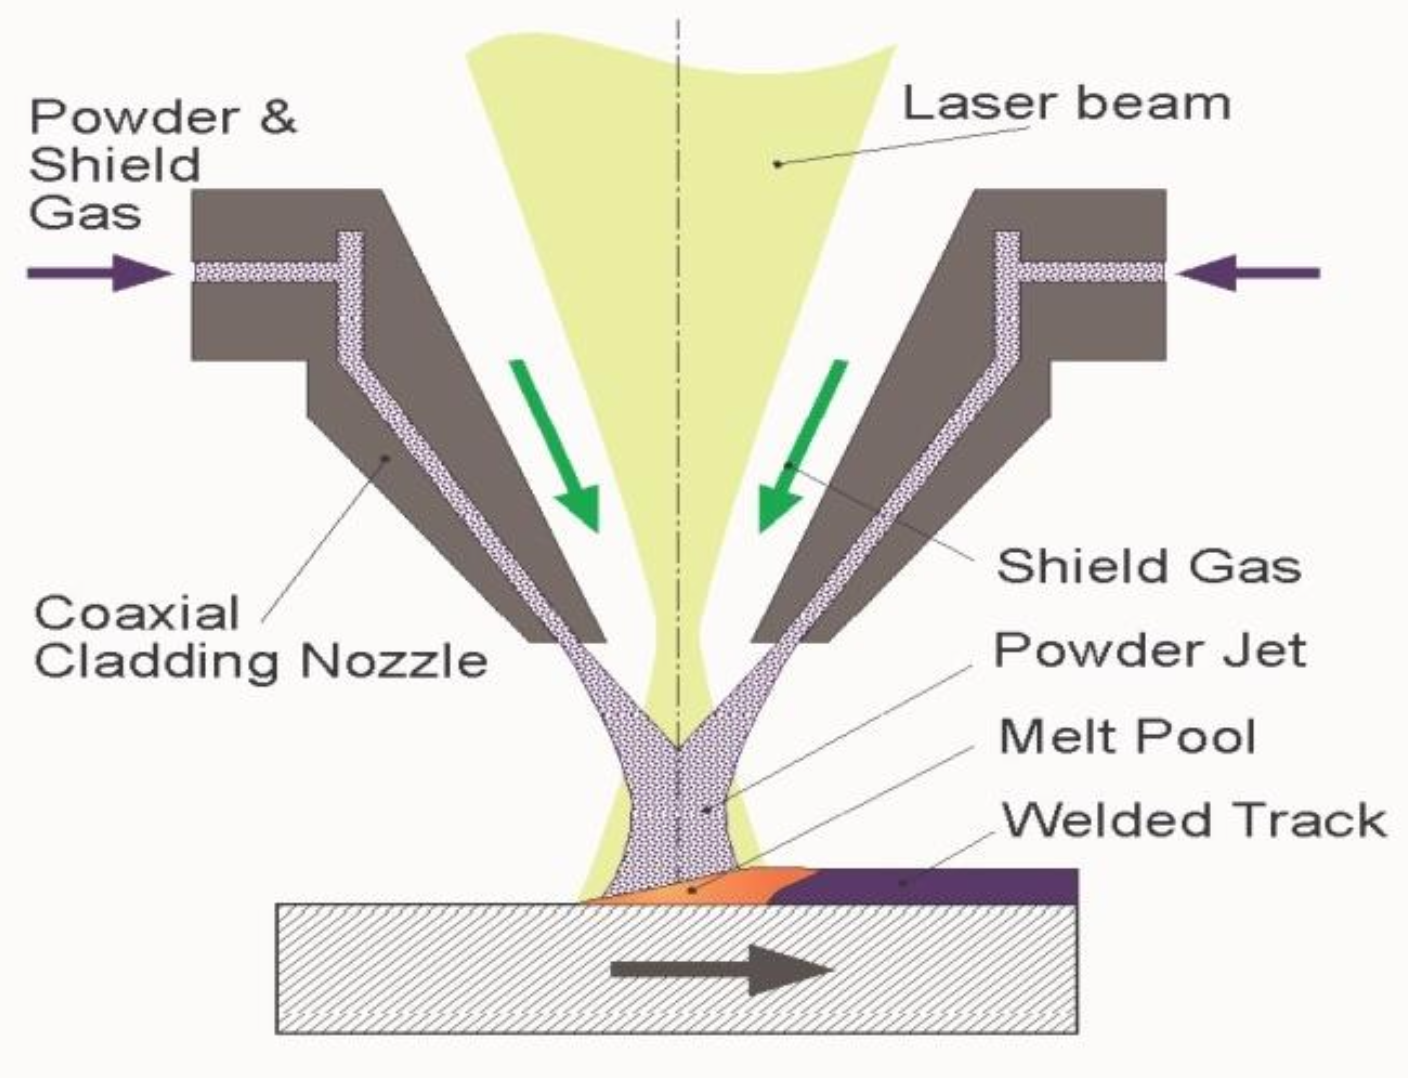
\includegraphics[width=0.5\textwidth]{slike/ded.png}
    \caption{DED nozzle}
    \label{fig:ded}
\end{figure}

Both the additional material and the existing part are molten and metallurgically bonded. 
Overlapping weld seams create 3D-geometry. 
